\documentclass[tikz, border=5mm]{standalone}

\usetikzlibrary{arrows.meta,decorations.markings,fit,calc, positioning}

\definecolor{componentColor}{RGB}{210,210,210}
\definecolor{systemColor}{RGB}{230,230,230}

\tikzset{component/.append style={fill=componentColor, align=center, draw, minimum width=2cm, minimum height=1.5cm, rounded corners=.3cm}}
\tikzset{system/.style={component, fill=systemColor, rounded corners=0cm}}

\tikzstyle{arrow} = [-{Latex[scale=3.0]}]
\tikzset{arrowLabel/.append style={minimum height=.25cm, draw=none}}
\begin{document}

	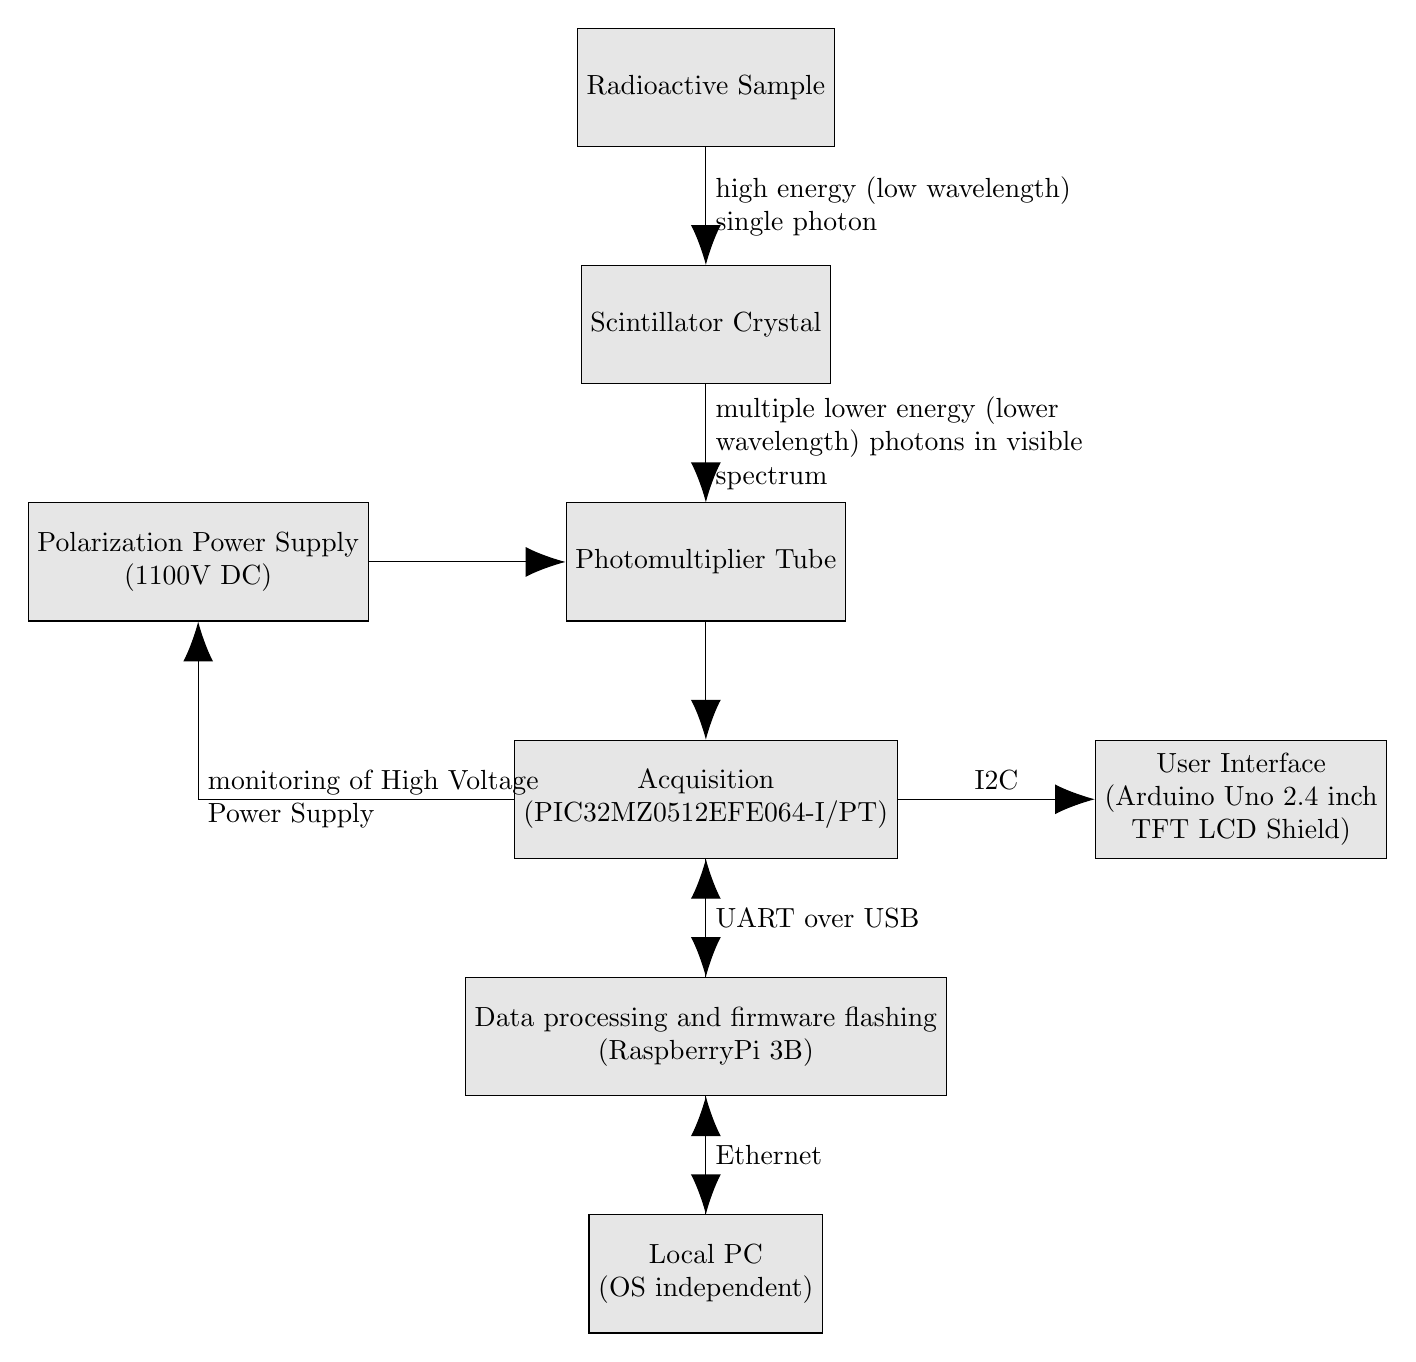
\begin{tikzpicture}[node distance=1.5cm and 2.5cm]
	% Nodes
	\pgfdeclarelayer{background}
	\pgfsetlayers{background,main}
	
		\node (sample) [system] {Radioactive Sample};
		\node (scintillator) [system, below=of sample] {Scintillator Crystal};
		
        \node (photomultiplier) [system, below=of scintillator] {Photomultiplier Tube};	
		\node (hwpower) [system, left=of photomultiplier] {Polarization Power Supply\\ (1100V DC)};
	
		\node (cpu) [system, below=of photomultiplier] {Acquisition\\ (PIC32MZ0512EFE064-I/PT)};
		\node (gui) [system, right=of cpu] {User Interface\\ (Arduino Uno 2.4 inch \\ TFT LCD Shield)};		

		\node (pi) [system, below=of cpu] {Data processing and firmware flashing\\ (RaspberryPi 3B)};
		\node (pc) [system, below=of pi] {Local PC\\ (OS independent)};
	    

		% Connectors
		\begin{scope}[->]
		
		\draw [arrow] (sample) -- node[anchor=west, minimum width=.25cm, draw=none, text width=5.0cm] 
			{high energy (low wavelength) single photon} (scintillator);

		\draw [arrow] (scintillator) -- node[anchor=west, minimum width=.25cm, draw=none, text width=5.0cm] 
			{multiple lower energy (lower wavelength) photons in visible spectrum} (photomultiplier);

		\draw [arrow] (hwpower) -- node[anchor=south, minimum width=.25cm, draw=none] {} (photomultiplier);

        \draw [arrow] (photomultiplier) -- (cpu);

		\draw [arrow] (cpu) -- node[anchor=south, minimum height=.25cm, draw=none] {I2C} (gui);

        \draw[arrow] (cpu.west) -- ++(0,0) -| node[anchor=west, minimum width=.25cm, draw=none, text width=5.0cm]{monitoring of High Voltage Power Supply} (hwpower.south); 

		\draw [arrow] (cpu) -- node[anchor=west, minimum height=.25cm, draw=none] {UART over USB} (pi);
		\draw [arrow] (pi) -- node[anchor=south, minimum height=.25cm, draw=none] {} (cpu);

		\draw [arrow] (pi) -- node[anchor=west, minimum height=.25cm, draw=none] {Ethernet} (pc);
		\draw [arrow] (pc) -- node[anchor=west, minimum height=.25cm, draw=none] {} (pi);

	\end{scope}

\end{tikzpicture}
\end{document}